\newpage
\subsection{Caso d'uso UC10 - Visualizzazione API registrate}
\label{UC10}
\begin{figure}[ht]
	\centering
	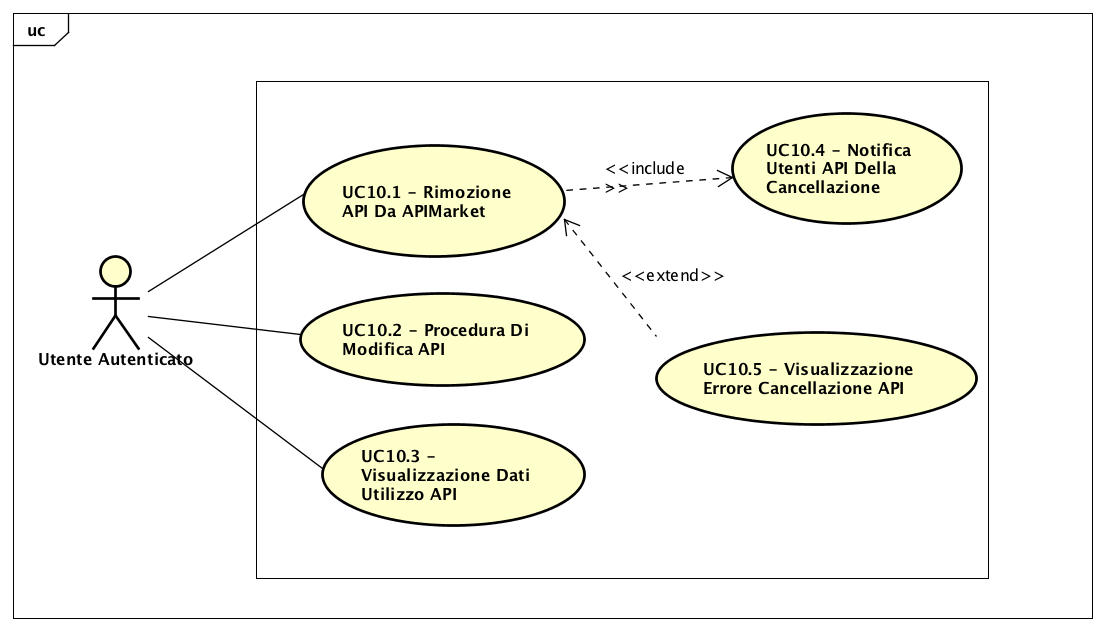
\includegraphics[scale=0.45]{UML/UC10.png}
	\caption{UC10: Visualizzazione API registrate}
\end{figure}

\begin{longtable}{ l | p{11cm}}
	\hline
	\rowcolor{Gray}
	\multicolumn{2}{c}{UC10 - Visualizzazione API registrate}\\
	\hline
	\textbf{Attori} & Utente autenticato, Amministratore API Market \\
	\textbf{Descrizione} & L'attore visualizza le API da lui registrate \\
	\textbf{Pre-Condizioni} & L'attore si trova nella schermata relativa alle API da lui registrate  \\
	\textbf{Post-Condizioni} & L'attore ha visualizzato le API da lui registrate \\
	\textbf{Scenario Principale} & 
	\begin{enumerate*}[label=(\arabic*.),itemjoin={\newline}]
		\item L'attore può visualizzare il numero delle API registrate (UC10.1)
		\item L'attore può visualizzare la lista delle API registrate (UC10.2)
	\end{enumerate*}\\
	\textbf{Scenari Alternativi} & 
	\begin{enumerate*}[label=(\arabic*.),itemjoin={\newline}]
		\item L'attore può visualizzare i dati relativi ad una singola API (UC7)
	\end{enumerate*}\\
\end{longtable}

\subsubsection{Caso d'uso UC10.1: Visualizzazione numero API registrate}
\label{UC10_1}

\begin{minipage}{\linewidth}
	\begin{tabular}{ l | p{11cm}}
		\hline
		\rowcolor{Gray}
		\multicolumn{2}{c}{UC10.1 - Visualizzazione numero API registrate} \\
		\hline
		\textbf{Attori} & Utente autenticato, Amministratore API Market \\
		\textbf{Descrizione} & L'attore visualizza il numero di API da lui registrate \\
		\textbf{Pre-Condizioni} & L'attore si trova nella schermata relativa alle API da lui registrate \\
		\textbf{Post-Condizioni} & L'attore ha visualizzato il numero delle API da lui registrate \\
		\textbf{Scenario Principale} & 
		\begin{enumerate*}[label=(\arabic*.),itemjoin={\newline}]
			\item L'attore può visualizzare il numero di API da lui registrate
		\end{enumerate*}\\
	\end{tabular}
\end{minipage}

\newpage
\subsubsection{Caso d'uso UC10.2: Visualizzazione lista API registrate}
\label{UC10_2}
\begin{figure}[ht]
	\centering
	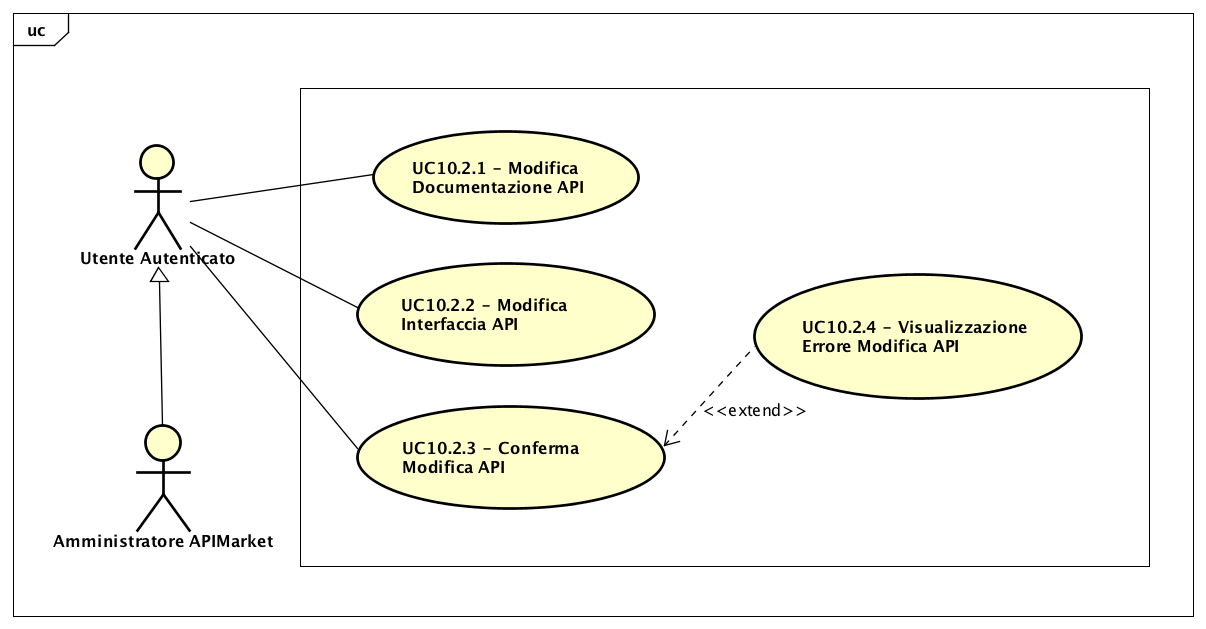
\includegraphics[scale=0.45]{UML/UC10_2.png}
	\caption{UC10.2: Visualizzazione lista API registrate}
\end{figure}

\begin{minipage}{\linewidth}
	\begin{tabular}{ l | p{11cm}}
		\hline
		\rowcolor{Gray}
		\multicolumn{2}{c}{UC10.2 - Visualizzazione lista API registrate} \\
		\hline
		\textbf{Attori} & Utente autenticato, Amministratore API Market \\
		\textbf{Descrizione} & L'attore visualizza la lista di ogni API da lui registrata \\
		\textbf{Pre-Condizioni} & L'attore si trova nella schermata relativa alle API da lui registrate \\
		\textbf{Post-Condizioni} & L'attore ha visualizzato la lista delle API da lui registrate \\
		\textbf{Scenario Principale} & 
		\begin{enumerate*}[label=(\arabic*.),itemjoin={\newline}]
			\item L'attore può visualizzare il nome di ogni API da lui registrata (UC10.2.1)
			\item L'attore può visualizzare il link alla pagina di visualizzazione API di ogni API da lui registrata (UC10.2.2)
			\item L'attore può visualizzare il numero di licenze attive di ogni API da lui registrata (UC10.2.3)
			\item L'attore può modificare ogni API da lui registrata (UC10.2.4)
			\item L'attore può eliminare ogni API da lui registrata (UC10.2.5)
		\end{enumerate*}\\
	\end{tabular}
\end{minipage}

\paragraph{Caso d'uso UC10.2.1: Visualizzazione nome API}
\label{UC10_2_1}

\begin{minipage}{\linewidth}
	\begin{tabular}{ l | p{11cm}}
		\hline
		\rowcolor{Gray}
		\multicolumn{2}{c}{UC10.2.1 - Visualizzazione nome API} \\
		\hline
		\textbf{Attori} & Utente autenticato, Amministratore API Market \\
		\textbf{Descrizione} & L'attore visualizza nella lista il nome di ogni API da lui registrata \\
		\textbf{Pre-Condizioni} & L'attore si trova nella schermata relativa alle API da lui registrate \\
		\textbf{Post-Condizioni} & L'attore ha visualizzato nella lista il nome di ogni API da lui registrata \\
		\textbf{Scenario Principale} & 
		\begin{enumerate*}[label=(\arabic*.),itemjoin={\newline}]
			\item L'attore può visualizzare nella lista il nome di ogni API da lui registrata
		\end{enumerate*}\\
	\end{tabular}
\end{minipage}

\paragraph{Caso d'uso UC10.2.2: Visualizzazione link API}
\label{UC10_2_2}

\begin{minipage}{\linewidth}
	\begin{tabular}{ l | p{11cm}}
		\hline
		\rowcolor{Gray}
		\multicolumn{2}{c}{UC10.2.2 - Visualizzazione link API} \\
		\hline
		\textbf{Attori} & Utente autenticato, Amministratore API Market \\
		\textbf{Descrizione} & L'attore visualizza nella lista il link alla visualizzazione di ogni API da lui registrata \\
		\textbf{Pre-Condizioni} & L'attore si trova nella schermata relativa alle API da lui registrate \\
		\textbf{Post-Condizioni} & L'attore ha visualizzato nella lista il link alla visualizzazione di ogni API da lui registrata \\
		\textbf{Scenario Principale} & 
		\begin{enumerate*}[label=(\arabic*.),itemjoin={\newline}]
			\item L'attore può visualizzare nella lista il link alla visualizzazione di ogni API da lui registrata
		\end{enumerate*}\\
	\end{tabular}
\end{minipage}

\paragraph{Caso d'uso UC10.2.3: Visualizzazione numero licenze attive}
\label{UC10_2_3}

\begin{minipage}{\linewidth}
	\begin{tabular}{ l | p{11cm}}
		\hline
		\rowcolor{Gray}
		\multicolumn{2}{c}{UC10.2.3 - Visualizzazione numero licenze attive} \\
		\hline
		\textbf{Attori} & Utente autenticato, Amministratore API Market \\
		\textbf{Descrizione} & L'attore visualizza nella lista il numero di licenze attive per ogni API da lui registrata \\
		\textbf{Pre-Condizioni} & L'attore si trova nella schermata relativa alle API da lui registrate \\
		\textbf{Post-Condizioni} & L'attore ha visualizzato nella lista il numero di licenze attive per ogni API da lui registrata \\
		\textbf{Scenario Principale} & 
		\begin{enumerate*}[label=(\arabic*.),itemjoin={\newline}]
			\item L'attore può visualizzare nella lista il numero di licenze attive per ogni API da lui registrata
		\end{enumerate*}\\
	\end{tabular}
\end{minipage}

\paragraph{Caso d'uso UC10.2.4: Notifica eliminazione API}
\label{UC10_2_1}

\begin{minipage}{\linewidth}
	\begin{tabular}{ l | p{11cm}}
		\hline
		\rowcolor{Gray}
		\multicolumn{2}{c}{UC10.2.1 - Notifica eliminazione API} \\
		\hline
		\textbf{Attori} & Utente autenticato, Amministratore API Market \\
		\textbf{Descrizione} & Per ogni API da lui registrata nella lista, l'attore visualizza se questa sia in fase di eliminazione \\
		\textbf{Pre-Condizioni} & L'attore si trova nella schermata relativa alle API da lui registrate \\
		\textbf{Post-Condizioni} & Per ogni API da lui registrata nella lista, l'attore ha visualizzato se questa sia in fase di eliminazione \\
		\textbf{Scenario Principale} & 
		\begin{enumerate*}[label=(\arabic*.),itemjoin={\newline}]
			\item Per ogni API da lui registrata nella lista, l'attore può visualizzare se questa sia in fase di eliminazione
		\end{enumerate*}\\
	\end{tabular}
\end{minipage}

\newpage
\paragraph{Caso d'uso UC10.2.5: Modifica API registrata}
\label{UC10_2_5}
\begin{figure}[ht]
	\centering
	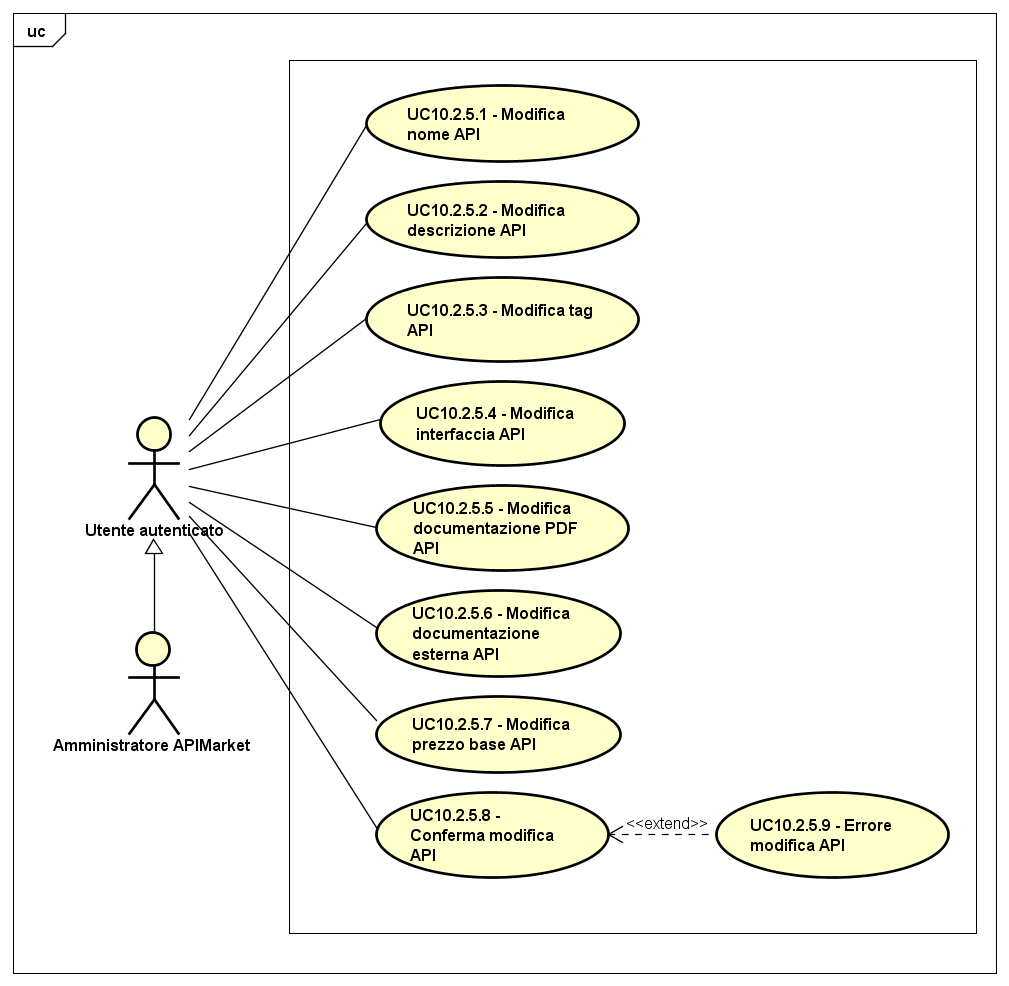
\includegraphics[scale=0.45]{UML/UC10_2_5.png}
	\caption{UC10.2.5: Modifica API registrata}
\end{figure}

\begin{minipage}{\linewidth}
	\begin{tabular}{ l | p{11cm}}
		\hline
		\rowcolor{Gray}
		\multicolumn{2}{c}{UC10.2.5 - Modifica API registrata} \\
		\hline
		\textbf{Attori} & Utente autenticato, Amministratore API Market \\
		\textbf{Descrizione} & L'attore modifica una API da lui registrata \\
		\textbf{Pre-Condizioni} & L'attore si trova nella schermata relativa alle API da lui registrate \\
		\textbf{Post-Condizioni} & L'attore ha modificato un API registrata \\
		\textbf{Scenario Principale} & 
		\begin{enumerate*}[label=(\arabic*.),itemjoin={\newline}]
			\item L'attore può modificare il nome dell'API (UC10.2.5.1)
			\item L'attore può modificare la descrizione dell'API (UC10.2.5.2)
			\item L'attore può modificare i tag dell'API (UC10.2.5.3)
			\item L'attore può modificare l'interfaccia dell'API (UC10.2.5.4)
			\item L'attore può modificare il file di documentazione PDF (UC10.2.5.5)
			\item L'attore può modificare il link alla documentazione esterna (UC10.2.5.6)
			\item L'attore può modificare il prezzo base dell'API (UC10.2.5.7)
			\item L'attore può confermare la modifica dell'API (UC10.2.5.8)
		\end{enumerate*}\\
		\textbf{Scenari Alternativi} & 
		\begin{enumerate*}[label=(\arabic*.),itemjoin={\newline}]
			\item L'attore può visualizzare un messaggio d'errore informativo e le modifiche non avvengono
		\end{enumerate*}\\
	\end{tabular}
\end{minipage}

\subparagraph{Caso d'uso UC10.2.5.1: Modifica nome API}
\label{UC10_2_5_1}

\begin{minipage}{\linewidth}
	\begin{tabular}{ l | p{11cm}}
		\hline
		\rowcolor{Gray}
		\multicolumn{2}{c}{UC10.2.5.1 - Modifica nome API} \\
		\hline
		\textbf{Attori} & Utente autenticato, Amministratore API Market \\
		\textbf{Descrizione} & L'attore modifica il nome dell'API \\
		\textbf{Pre-Condizioni} & L'attore si trova nella schermata relativa alla modifica di una API registrata, precedentemente selezionata \\
		\textbf{Post-Condizioni} & L'attore ha modificato il nome dell'API selezionata \\
		\textbf{Scenario Principale} & 
		\begin{enumerate*}[label=(\arabic*.),itemjoin={\newline}]
			\item L'attore può modificare il nome dell'API
		\end{enumerate*}\\
	\end{tabular}
\end{minipage}

\subparagraph{Caso d'uso UC10.2.5.2: Modifica descrizione API}
\label{UC10_2_5_2}

\begin{minipage}{\linewidth}
	\begin{tabular}{ l | p{11cm}}
		\hline
		\rowcolor{Gray}
		\multicolumn{2}{c}{UC10.2.5.2 - Modifica descrizione API} \\
		\hline
		\textbf{Attori} & Utente autenticato, Amministratore API Market \\
		\textbf{Descrizione} & L'attore modifica la descrizione dell'API\\
		\textbf{Pre-Condizioni} & L'attore si trova nella schermata relativa alla modifica di una API registrata, precedentemente selezionata \\
		\textbf{Post-Condizioni} & L'attore ha modificato la descrizione dell'API selezionata \\
		\textbf{Scenario Principale} & 
		\begin{enumerate*}[label=(\arabic*.),itemjoin={\newline}]
			\item L'attore può modificare la descrizione dell'API
		\end{enumerate*}\\
	\end{tabular}
\end{minipage}

\subparagraph{Caso d'uso UC10.2.5.3: Modifica tag API}
\label{UC10_2_5_3}

\begin{minipage}{\linewidth}
	\begin{tabular}{ l | p{11cm}}
		\hline
		\rowcolor{Gray}
		\multicolumn{2}{c}{UC10.2.5.3 - Modifica tag API} \\
		\hline
		\textbf{Attori} & Utente autenticato, Amministratore API Market \\
		\textbf{Descrizione} & L'attore modifica i tag dell'API \\
		\textbf{Pre-Condizioni} & L'attore si trova nella schermata relativa alla modifica di una API registrata, precedentemente selezionata \\
		\textbf{Post-Condizioni} & L'attore ha modificato i tag dell'API selezionata \\
		\textbf{Scenario Principale} & 
		\begin{enumerate*}[label=(\arabic*.),itemjoin={\newline}]
			\item L'attore può modificare i tag dell'API
		\end{enumerate*}\\
	\end{tabular}
\end{minipage}

\subparagraph{Caso d'uso UC10.2.5.4: Modifica interfaccia API}
\label{UC10_2_5_4}

\begin{minipage}{\linewidth}
	\begin{tabular}{ l | p{11cm}}
		\hline
		\rowcolor{Gray}
		\multicolumn{2}{c}{UC10.2.5.4 - Modifica interfaccia API} \\
		\hline
		\textbf{Attori} & Utente autenticato, Amministratore API Market \\
		\textbf{Descrizione} & L'attore modifica l'interfaccia dell'API \\
		\textbf{Pre-Condizioni} & L'attore si trova nella schermata relativa alla modifica di una API registrata, precedentemente selezionata \\
		\textbf{Post-Condizioni} & L'attore ha modificato l'interfaccia pubblica dell'API selezionata \\
		\textbf{Scenario Principale} & 
		\begin{enumerate*}[label=(\arabic*.),itemjoin={\newline}]
			\item L'attore può modificare l'interfaccia pubblica dell'API
		\end{enumerate*}\\
	\end{tabular}
\end{minipage}

\subparagraph{Caso d'uso UC10.2.5.5: Modifica documentazione PDF API}
\label{UC10_2_5_5}

\begin{minipage}{\linewidth}
	\begin{tabular}{ l | p{11cm}}
		\hline
		\rowcolor{Gray}
		\multicolumn{2}{c}{UC10.2.5.5 - Modifica documentazione PDF API} \\
		\hline
		\textbf{Attori} & Utente autenticato, Amministratore API Market \\
		\textbf{Descrizione} & L'attore modifica la documentazione PDF dell'API \\
		\textbf{Pre-Condizioni} & L'attore si trova nella schermata relativa alla modifica di una API registrata, precedentemente selezionata \\
		\textbf{Post-Condizioni} & L'attore ha modificato il file di documentazione dell'API selezionata \\
		\textbf{Scenario Principale} & 
		\begin{enumerate*}[label=(\arabic*.),itemjoin={\newline}]
			\item L'attore può selezionare un nuovo file dalle sue cartelle personali, che verrà caricato alla conferma
		\end{enumerate*}\\
		\textbf{Scenario Principale} & 
		\begin{enumerate*}[label=(\arabic*.),itemjoin={\newline}]
			\item Il file selezionato è di un formato non conforme e l'operazione non avviene
		\end{enumerate*}\\
	\end{tabular}
\end{minipage}

\subparagraph{Caso d'uso UC10.2.5.6: Modifica documentazione esterna API}
\label{UC10_2_5_6}

\begin{minipage}{\linewidth}
	\begin{tabular}{ l | p{11cm}}
		\hline
		\rowcolor{Gray}
		\multicolumn{2}{c}{UC10.2.5.6 - Modifica documentazione esterna API} \\
		\hline
		\textbf{Attori} & Utente autenticato, Amministratore API Market \\
		\textbf{Descrizione} & L'attore modifica la documentazione esterna dell'API \\
		\textbf{Pre-Condizioni} & L'attore si trova nella schermata relativa alla modifica di una API registrata, precedentemente selezionata \\
		\textbf{Post-Condizioni} & L'attore ha modificato il link di documentazione esterna dell'API selezionata \\
		\textbf{Scenario Principale} & 
		\begin{enumerate*}[label=(\arabic*.),itemjoin={\newline}]
			\item L'attore può modificare il link di documentazione esterna dell'API
		\end{enumerate*}\\
	\end{tabular}
\end{minipage}

\subparagraph{Caso d'uso UC10.2.5.7: Modifica prezzo base API}
\label{UC10_2_5_7}

\begin{minipage}{\linewidth}
	\begin{tabular}{ l | p{11cm}}
		\hline
		\rowcolor{Gray}
		\multicolumn{2}{c}{UC10.2.5.7 - Modifica prezzo base API} \\
		\hline
		\textbf{Attori} & Utente autenticato, Amministratore API Market \\
		\textbf{Descrizione} & L'attore modifica il prezzo base dell'API \\
		\textbf{Pre-Condizioni} & L'attore si trova nella schermata relativa alla modifica di una API registrata, precedentemente selezionata \\
		\textbf{Post-Condizioni} & L'attore ha modificato prezzo base dell'API selezionata \\
		\textbf{Scenario Principale} & 
		\begin{enumerate*}[label=(\arabic*.),itemjoin={\newline}]
			\item L'attore può modificare prezzo base dell'API
		\end{enumerate*}\\
	\end{tabular}
\end{minipage}

\subparagraph{Caso d'uso UC10.2.5.8: Conferma modifica API}
\label{UC10_2_5_8}

\begin{minipage}{\linewidth}
	\begin{tabular}{ l | p{11cm}}
		\hline
		\rowcolor{Gray}
		\multicolumn{2}{c}{UC10.2.5.8 - Conferma modifica API} \\
		\hline
		\textbf{Attori} & Utente autenticato, Amministratore API Market \\
		\textbf{Descrizione} & L'attore conferma le modifiche all'API, visualizzando un messaggio di successo \\
		\textbf{Pre-Condizioni} & L'attore si trova nella schermata relativa alla modifica di una API registrata, precedentemente selezionata \\
		\textbf{Post-Condizioni} & L'attore ha confermato le modifiche all'API, visualizzando un messaggio di successo \\
		\textbf{Scenario Principale} & 
		\begin{enumerate*}[label=(\arabic*.),itemjoin={\newline}]
			\item L'attore può confermare le modifiche effettuate all'API, visualizzando un messaggio di successo e venendo reindirizzato alla schermata di visualizzazione API registrate (UC10)
		\end{enumerate*}\\
	\end{tabular}
\end{minipage}

\subparagraph{Caso d'uso UC10.2.5.9: Errore modifica API}
\label{UC10_2_5_9}

\begin{minipage}{\linewidth}
	\begin{tabular}{ l | p{11cm}}
		\hline
		\rowcolor{Gray}
		\multicolumn{2}{c}{UC10.2.5.9 - Errore modifica API} \\
		\hline
		\textbf{Attori} & Utente autenticato, Amministratore API Market \\
		\textbf{Descrizione} & L'attore visualizza un messaggio di errore e la modifica non avviene \\
		\textbf{Pre-Condizioni} & L'attore ha confermato la modifica di una API ma si è verificato un errore \\
		\textbf{Post-Condizioni} & L'attore ha visualizzato un errore relativo alla modifica dell'API, con opportuna descrizione \\
		\textbf{Scenario Principale} & 
		\begin{enumerate*}[label=(\arabic*.),itemjoin={\newline}]
			\item L'attore può visualizzare un messaggio di errore e la modifica non avviene
		\end{enumerate*}\\
	\end{tabular}
\end{minipage}

\paragraph{Caso d'uso UC10.2.6: Eliminazione API registrata}
\label{UC10_2_6}

\begin{minipage}{\linewidth}
	\begin{tabular}{ l | p{11cm}}
		\hline
		\rowcolor{Gray}
		\multicolumn{2}{c}{UC10.2.6 - Eliminazione API registrata} \\
		\hline
		\textbf{Attori} & Utente autenticato, Amministratore API Market \\
		\textbf{Descrizione} & L'attore richiede l'eliminazione di una API da lui registrata, che verrà eliminata secondo le politiche di API Market \\
		\textbf{Pre-Condizioni} & L'attore si trova nella schermata relativa alle API da lui registrate \\
		\textbf{Post-Condizioni} & L'attore ha richiesto l'eliminazione di una API da lui registrata \\
		\textbf{Scenario Principale} & 
		\begin{enumerate*}[label=(\arabic*.),itemjoin={\newline}]
			\item L'attore può richiedere l'eliminazione di una API da lui registrata, che verrà eliminata secondo le politiche di API Market
		\end{enumerate*}\\
	\end{tabular}
\end{minipage}

\paragraph{Caso d'uso UC10.2.7: Revoca eliminazione API registrata}
\label{UC10_2_7}

\begin{minipage}{\linewidth}
	\begin{tabular}{ l | p{11cm}}
		\hline
		\rowcolor{Gray}
		\multicolumn{2}{c}{UC10.2.7 - Revoca eliminazione API registrata} \\
		\hline
		\textbf{Attori} & Utente autenticato, Amministratore API Market \\
		\textbf{Descrizione} & L'attore revoca la richiesta di eliminazione di una API da lui registrata \\
		\textbf{Pre-Condizioni} & L'attore si trova nella schermata relativa alle API da lui registrate \\
		\textbf{Post-Condizioni} & L'attore ha revocato la richiesta di eliminazione di una API da lui registrata \\
		\textbf{Scenario Principale} & 
		\begin{enumerate*}[label=(\arabic*.),itemjoin={\newline}]
			\item L'attore può revocare la richiesta di eliminazione di una API da lui registrata
		\end{enumerate*}\\
	\end{tabular}
\end{minipage}